\section{Luồng chat thường qua Rasa}

Luồng này mô tả trường hợp người dùng gửi một câu hỏi thông thường và hệ thống có thể xử lý trọn vẹn trong nhánh Rasa mà không cần chuyển sang RAG. Dữ liệu đi từ giao diện chat ở frontend, qua lớp Flask API trung gian, sau đó được chuyển tới Rasa để phân loại ý định, chọn rule hoặc action phù hợp và trả phản hồi về cho người dùng.

\begin{figure}[H]
    \centering
    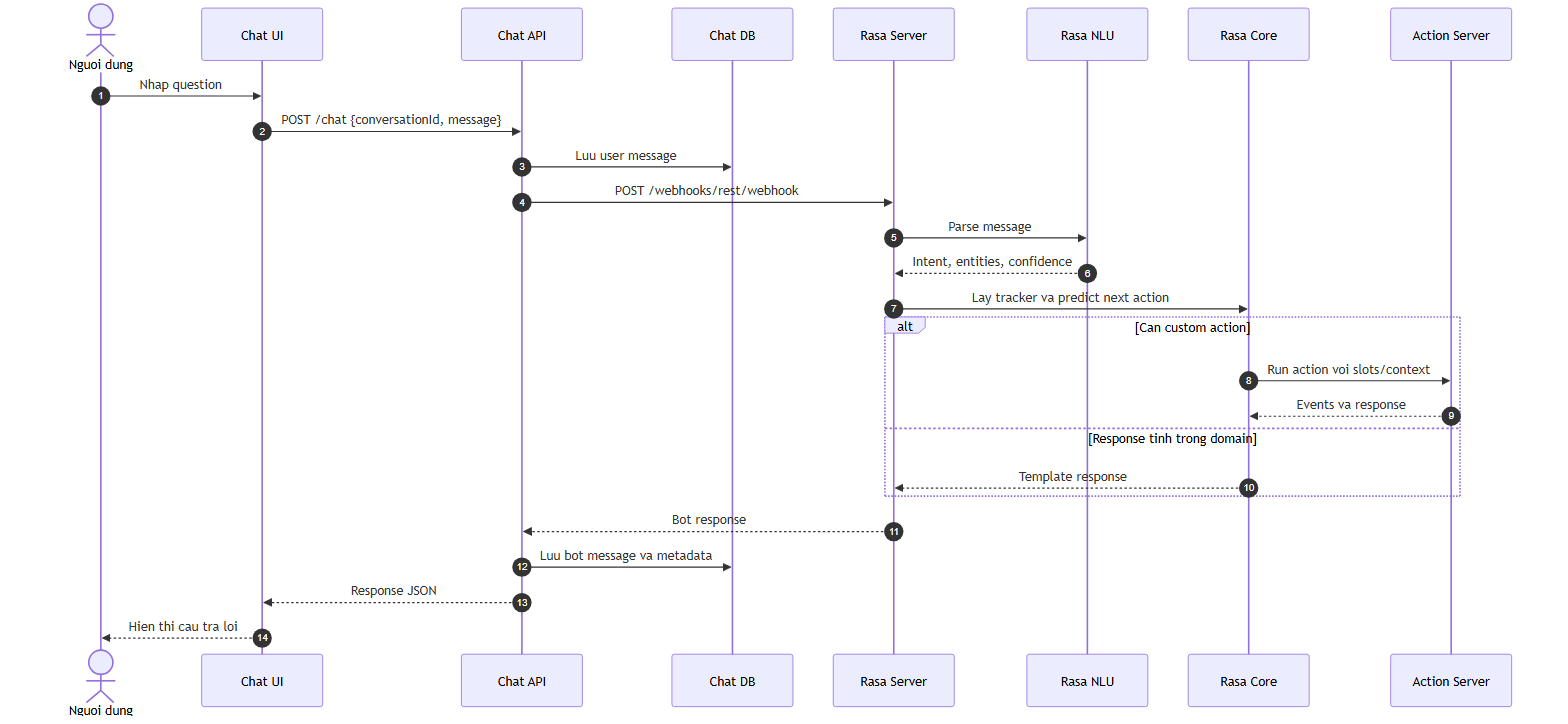
\includegraphics[width=\textwidth]{content/source/mermaid_sequence/seq_01.png}
    \caption{Luồng chat thường qua Rasa}
\end{figure}

Về mặt xử lý, frontend đóng vai trò thu thập nội dung câu hỏi và gắn với chatbot đang được chọn hoặc phiên hội thoại hiện tại. Flask API chuẩn hóa request, chuyển tiếp sang webhook REST của Rasa, sau đó gom các message phản hồi thành dữ liệu trả về cho giao diện. Trong Rasa, pipeline NLU nhận diện intent, entity và kích hoạt tầng quản lý hội thoại để suy ra response hoặc action tiếp theo. Khi intent có độ tin cậy đủ cao và rule tương ứng đã được định nghĩa, câu trả lời được tạo ra hoàn toàn trong nhánh này.
